\chapter{Requisitos e Arquitetura da Aplicação}
\label{chap:requisitos-arquitetura}

Este capítulo apresenta a visão funcional e arquitetural da JagozApp. Em
primeiro lugar são descritos os requisitos funcionais e não funcionais do
projeto, distinguindo entre funcionalidades obrigatórias e funcionalidades
complementares. De seguida é apresentada a arquitetura geral da aplicação, os
principais fluxos de utilização e as decisões arquiteturais que orientaram a
implementação.

\section{Visão Geral da Aplicação}

A JagozApp foi desenvolvida com o objetivo de centralizar a gestão operacional
de um clube desportivo local, reduzindo a dependência de processos manuais,
ficheiros dispersos e comunicação informal. A aplicação cobre várias áreas de
funcionamento do clube: gestão de sócios, inscrições de atletas, patrocínios,
eventos, bilhética, pagamentos, documentos e administração interna.

Do ponto de vista dos utilizadores, a aplicação distingue três perfis principais:

\begin{itemize}
    \item \textbf{Visitante}: utilizador não autenticado, com acesso a páginas
    públicas, informação institucional, consulta de atletas por escalão,
    informação de patrocínios e compra de bilhetes;
    \item \textbf{Utilizador autenticado}: utilizador com conta, que pode gerir
    o seu perfil, submeter pedidos, inscrever atletas, consultar patrocínios
    associados e realizar pagamentos;
    \item \textbf{Administração/Secretaria}: utilizador com permissões de
    gestão, responsável por aprovar pedidos, gerir sócios, atletas,
    patrocinadores, eventos, bilhetes, utilizadores e configurações.
\end{itemize}

A aplicação foi concebida como um sistema web completo, composto por uma
interface \textit{frontend}, uma API \textit{backend}, uma base de dados
relacional e integrações externas para pagamentos, correio eletrónico e
armazenamento de ficheiros.

\section{Requisitos Funcionais}

Os requisitos funcionais representam as funcionalidades que o sistema deve
disponibilizar aos seus utilizadores. Estes requisitos foram organizados por
domínio funcional.

\subsection{Requisitos Obrigatórios}

Os requisitos obrigatórios correspondem às funcionalidades essenciais para que
a aplicação cumpra o seu objetivo principal.

\begin{itemize}
    \item \textbf{Autenticação e gestão de utilizadores}: permitir o registo,
    início de sessão, fim de sessão e identificação do utilizador autenticado;
    \item \textbf{Autorização por papéis}: distinguir permissões entre
    utilizadores normais, secretaria e administradores;
    \item \textbf{Gestão de sócios}: permitir criar, consultar, editar,
    aprovar, rejeitar, reativar e desativar sócios;
    \item \textbf{Inscrição e gestão de atletas}: permitir a inscrição de
    atletas, incluindo dados pessoais, desportivos, escolares e encarregados de
    educação;
    \item \textbf{Consulta pública de atletas}: disponibilizar informação não
    sensível sobre atletas por escalão;
    \item \textbf{Gestão de equipas e escalões}: permitir configurar grupos,
    escalões e respetiva organização;
    \item \textbf{Gestão de patrocinadores}: permitir criar e consultar
    patrocinadores;
    \item \textbf{Gestão de patrocínios}: permitir submeter, aprovar, cancelar
    e marcar patrocínios como pagos;
    \item \textbf{Catálogo de patrocínios}: permitir configurar opções de
    publicidade, patrocínio de equipas e outros apoios;
    \item \textbf{Gestão de eventos}: permitir criar, consultar, editar e
    cancelar eventos;
    \item \textbf{Bilhética}: permitir a compra de bilhetes para eventos e a
    validação de condições de sócio quando aplicável;
    \item \textbf{Pagamentos}: permitir iniciar pagamentos online e registar o
    seu estado;
    \item \textbf{Recibos}: permitir consultar recibos de pagamentos e de
    patrocínios;
    \item \textbf{Gestão de ficheiros}: permitir carregar, consultar e remover
    documentos ou fotografias associados a entidades da aplicação;
    \item \textbf{Painel administrativo}: apresentar indicadores gerais sobre
    o estado do clube e acesso às áreas de gestão.
\end{itemize}

\subsection{Requisitos Complementares}

Para além das funcionalidades essenciais, foram identificados requisitos
complementares que aumentam a qualidade da solução e melhoram a experiência de
utilização.

\begin{itemize}
    \item \textbf{Internacionalização}: disponibilizar a interface em português
    e inglês;
    \item \textbf{Execução em Docker}: permitir correr a aplicação localmente
    através de containers;
    \item \textbf{Documentação da API}: disponibilizar uma especificação
    OpenAPI para consulta dos \textit{endpoints};
    \item \textbf{Testes automatizados}: validar regras de domínio,
    mapeamentos HTTP e serviços principais;
    \item \textbf{Notificações por email}: enviar confirmações associadas a
    fluxos como a compra de bilhetes;
    \item \textbf{Geração de códigos QR}: associar bilhetes confirmados a
    códigos QR para posterior validação;
    \item \textbf{Armazenamento externo de ficheiros}: guardar conteúdo binário
    fora da base de dados relacional.
\end{itemize}

\section{Requisitos Não Funcionais}

Os requisitos não funcionais definem propriedades de qualidade que a aplicação
deve respeitar.

\begin{itemize}
    \item \textbf{Manutenibilidade}: a aplicação deve estar organizada por
    módulos e camadas, facilitando alterações futuras;
    \item \textbf{Testabilidade}: a lógica de domínio e de serviços deve poder
    ser testada de forma isolada;
    \item \textbf{Segurança}: palavras-passe não devem ser guardadas em texto
    simples e o acesso a dados sensíveis deve exigir autenticação e autorização;
    \item \textbf{Privacidade}: dados sensíveis de sócios e atletas não devem
    ser expostos em páginas públicas;
    \item \textbf{Consistência}: operações que envolvem múltiplas entidades
    devem ser executadas dentro de transações;
    \item \textbf{Usabilidade}: a interface deve ser clara, organizada e
    adequada a utilizadores com diferentes níveis de conhecimento técnico;
    \item \textbf{Portabilidade}: o projeto deve poder ser executado em
    ambiente local através de Docker;
    \item \textbf{Escalabilidade evolutiva}: a arquitetura deve permitir a
    adição de novas funcionalidades sem reestruturações profundas.
\end{itemize}

\section{Arquitetura Geral}

A arquitetura da JagozApp segue uma separação clara entre cliente, servidor,
persistência e serviços externos. O \textit{frontend}, implementado em React,
é responsável pela interação com o utilizador. O \textit{backend}, implementado
em Kotlin com Spring Boot, expõe uma Web API REST e concentra a lógica de
negócio. A persistência dos dados estruturados é feita em PostgreSQL, enquanto
ficheiros, pagamentos e email são delegados a serviços externos.

\begin{figure}[H]
    \centering
    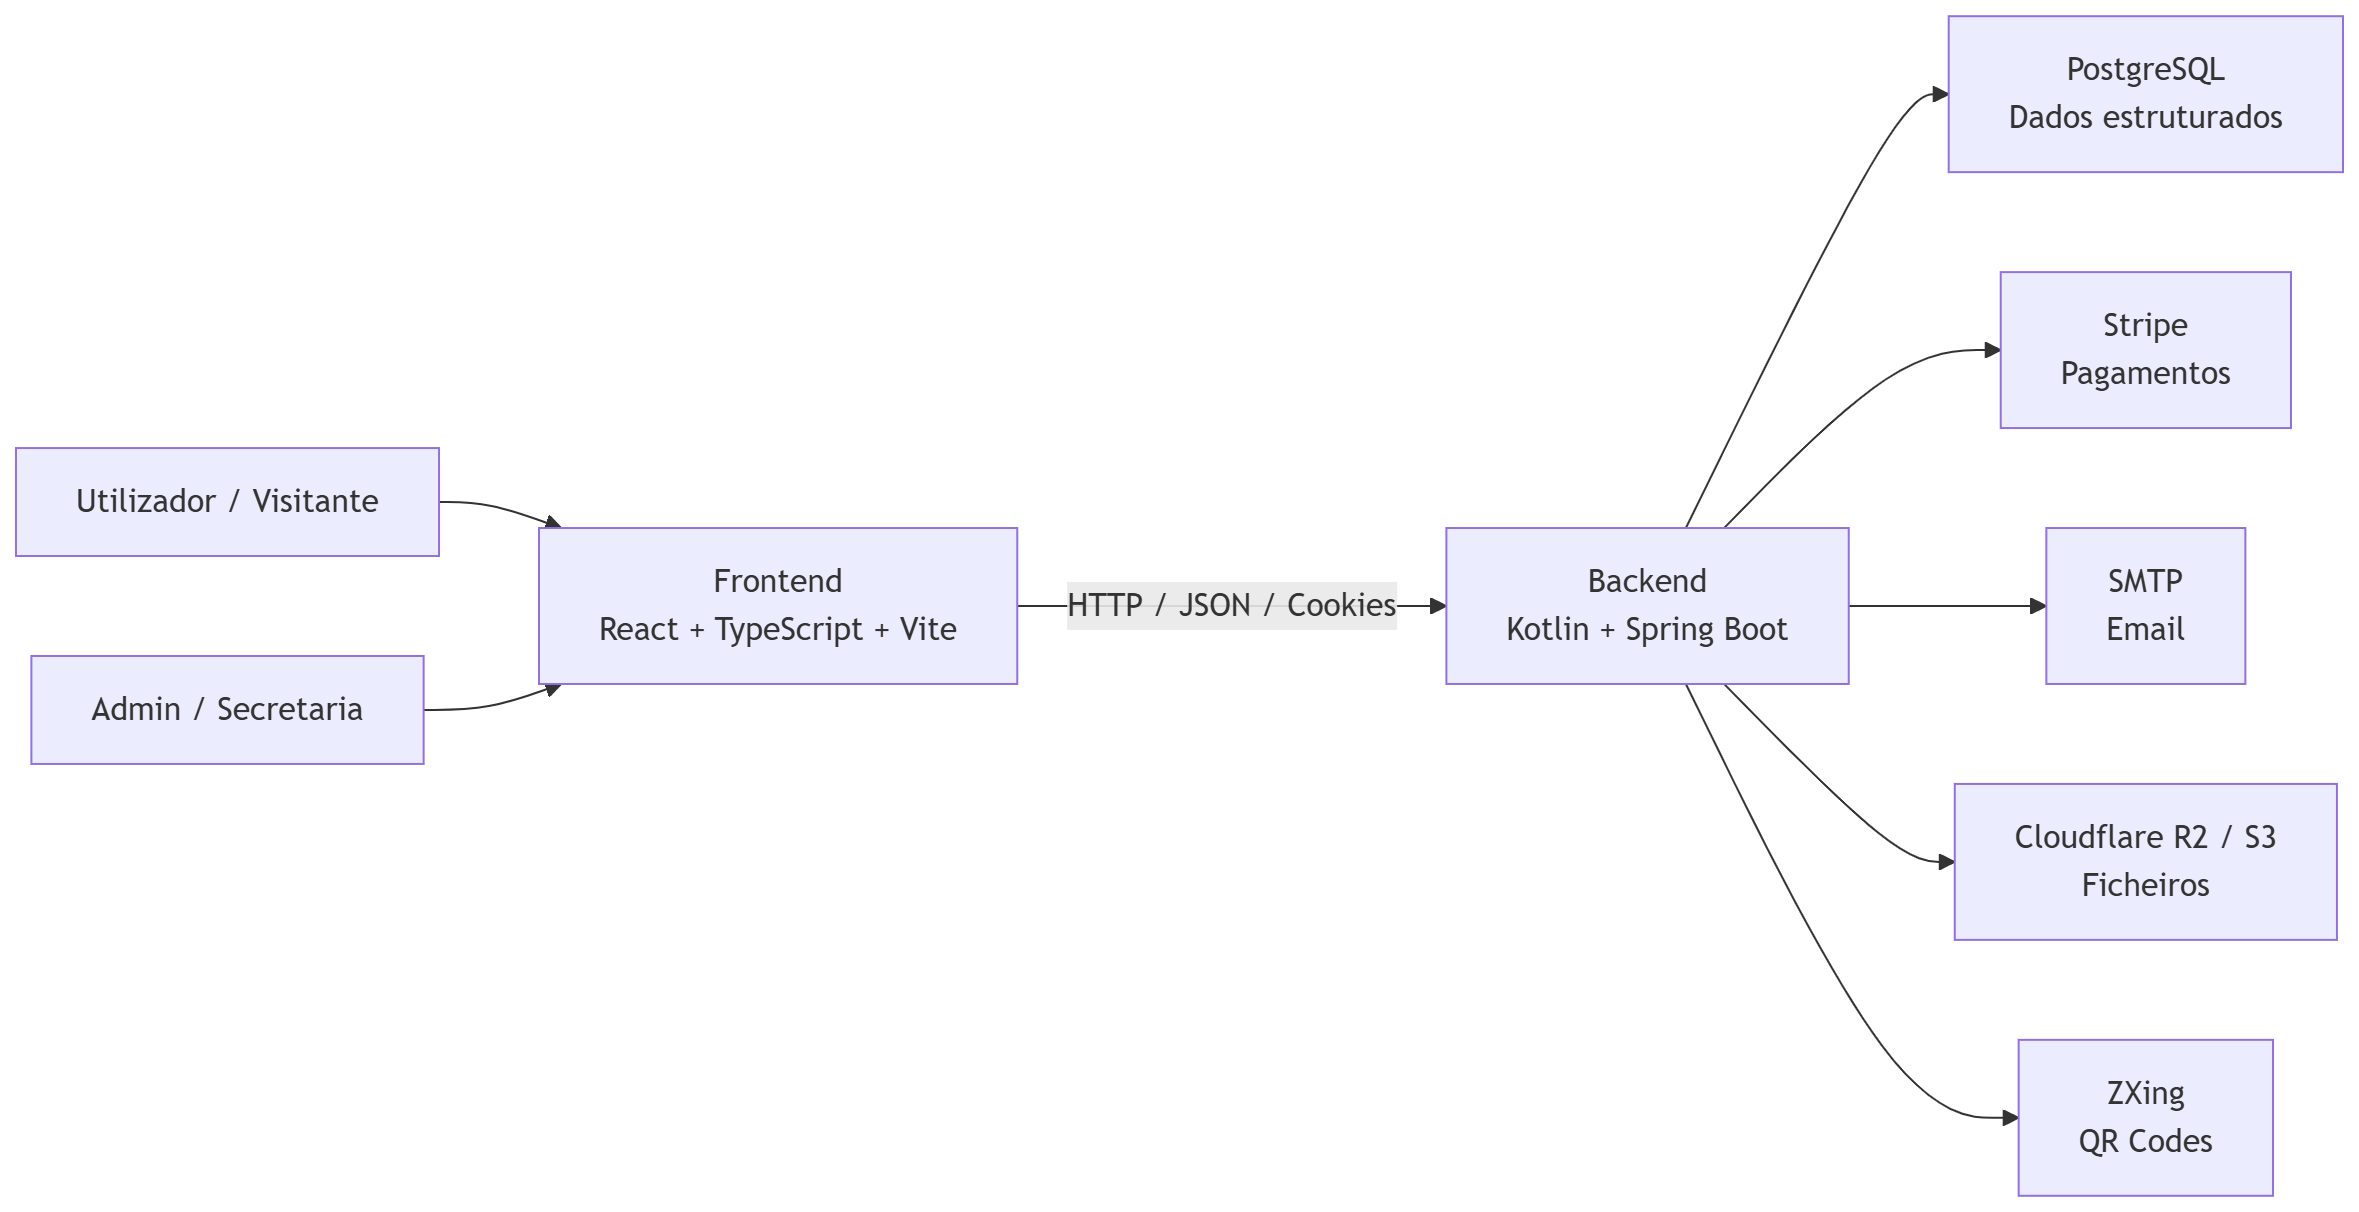
\includegraphics[width=\textwidth]{./figures/architecture-context.png}
    \caption{Arquitetura geral da aplicação}
    \label{fig:architecture-context}
\end{figure}

Esta divisão permite separar responsabilidades e reduzir o acoplamento entre
componentes. O \textit{frontend} não acede diretamente à base de dados, fazendo
todos os pedidos através da API. O \textit{backend}, por sua vez, concentra a
validação das regras de negócio e controla o acesso aos dados e integrações.

\section{Arquitetura Modular}

O projeto foi organizado como uma aplicação multi-módulo. Esta decisão foi
tomada para separar claramente as responsabilidades internas do sistema e
evitar que todas as classes ficassem concentradas num único módulo. Embora esta
separação seja mais visível no \textit{backend}, ela influencia a forma como a
aplicação é mantida e testada.

A organização em módulos permite:

\begin{itemize}
    \item isolar a lógica de domínio de detalhes tecnológicos;
    \item impedir que os controladores dependam diretamente da base de dados;
    \item substituir implementações de repositórios sem alterar os serviços;
    \item testar regras de negócio sem iniciar a aplicação completa;
    \item tornar explícitas as dependências entre camadas;
    \item facilitar a evolução futura do projeto.
\end{itemize}

Os principais módulos do \textit{backend} são:

\begin{itemize}
    \item \texttt{domain}: entidades, enumerações, validações e regras puras de
    domínio;
    \item \texttt{repository}: contratos de acesso a dados;
    \item \texttt{repository-jdbi}: implementação concreta dos repositórios em
    PostgreSQL através de JDBI;
    \item \texttt{services}: casos de uso e lógica de negócio da aplicação;
    \item \texttt{http}: controladores REST, modelos HTTP e pipeline de
    autenticação;
    \item \texttt{host}: módulo de arranque e configuração da aplicação Spring
    Boot.
\end{itemize}

\begin{figure}[H]
    \centering
    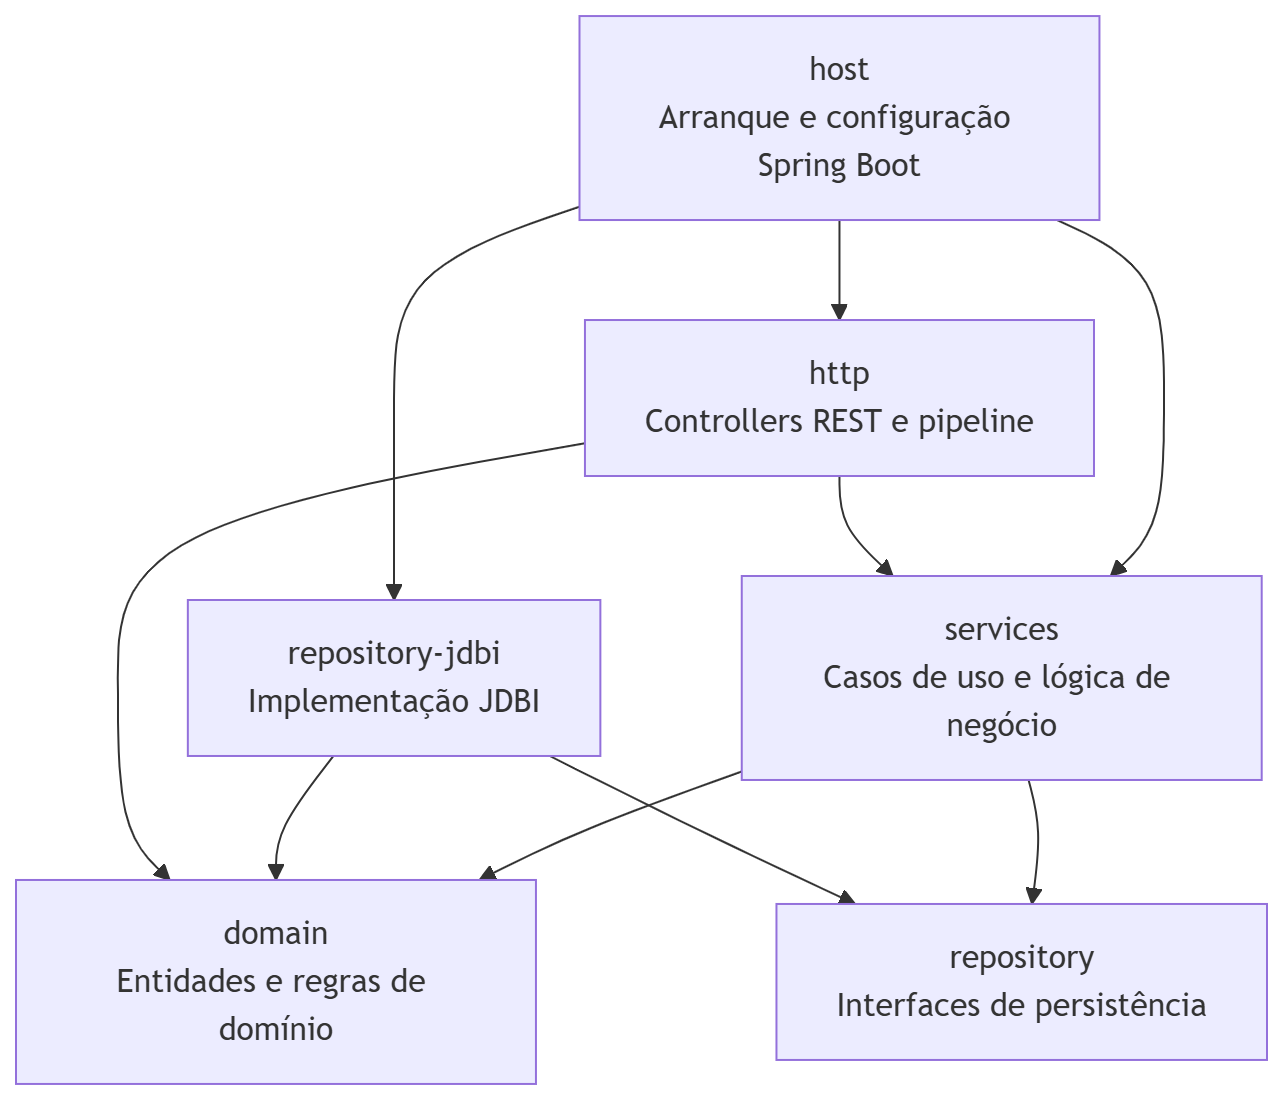
\includegraphics[width=\textwidth]{./figures/backend-modules.png}
    \caption{Dependências entre os módulos do backend}
    \label{fig:backend-modules}
\end{figure}

\section{Principais Fluxos da Aplicação}

Esta secção descreve os principais fluxos de utilização suportados pela
aplicação.

\subsection{Fluxo de Autenticação}

O fluxo de autenticação começa quando o utilizador submete as suas credenciais
no \textit{frontend}. O \textit{backend} valida a palavra-passe e, em caso de
sucesso, cria um \textit{token} de sessão. Esse \textit{token} é enviado ao
cliente através de um \textit{cookie} e usado nos pedidos seguintes.

\begin{figure}[H]
    \centering
    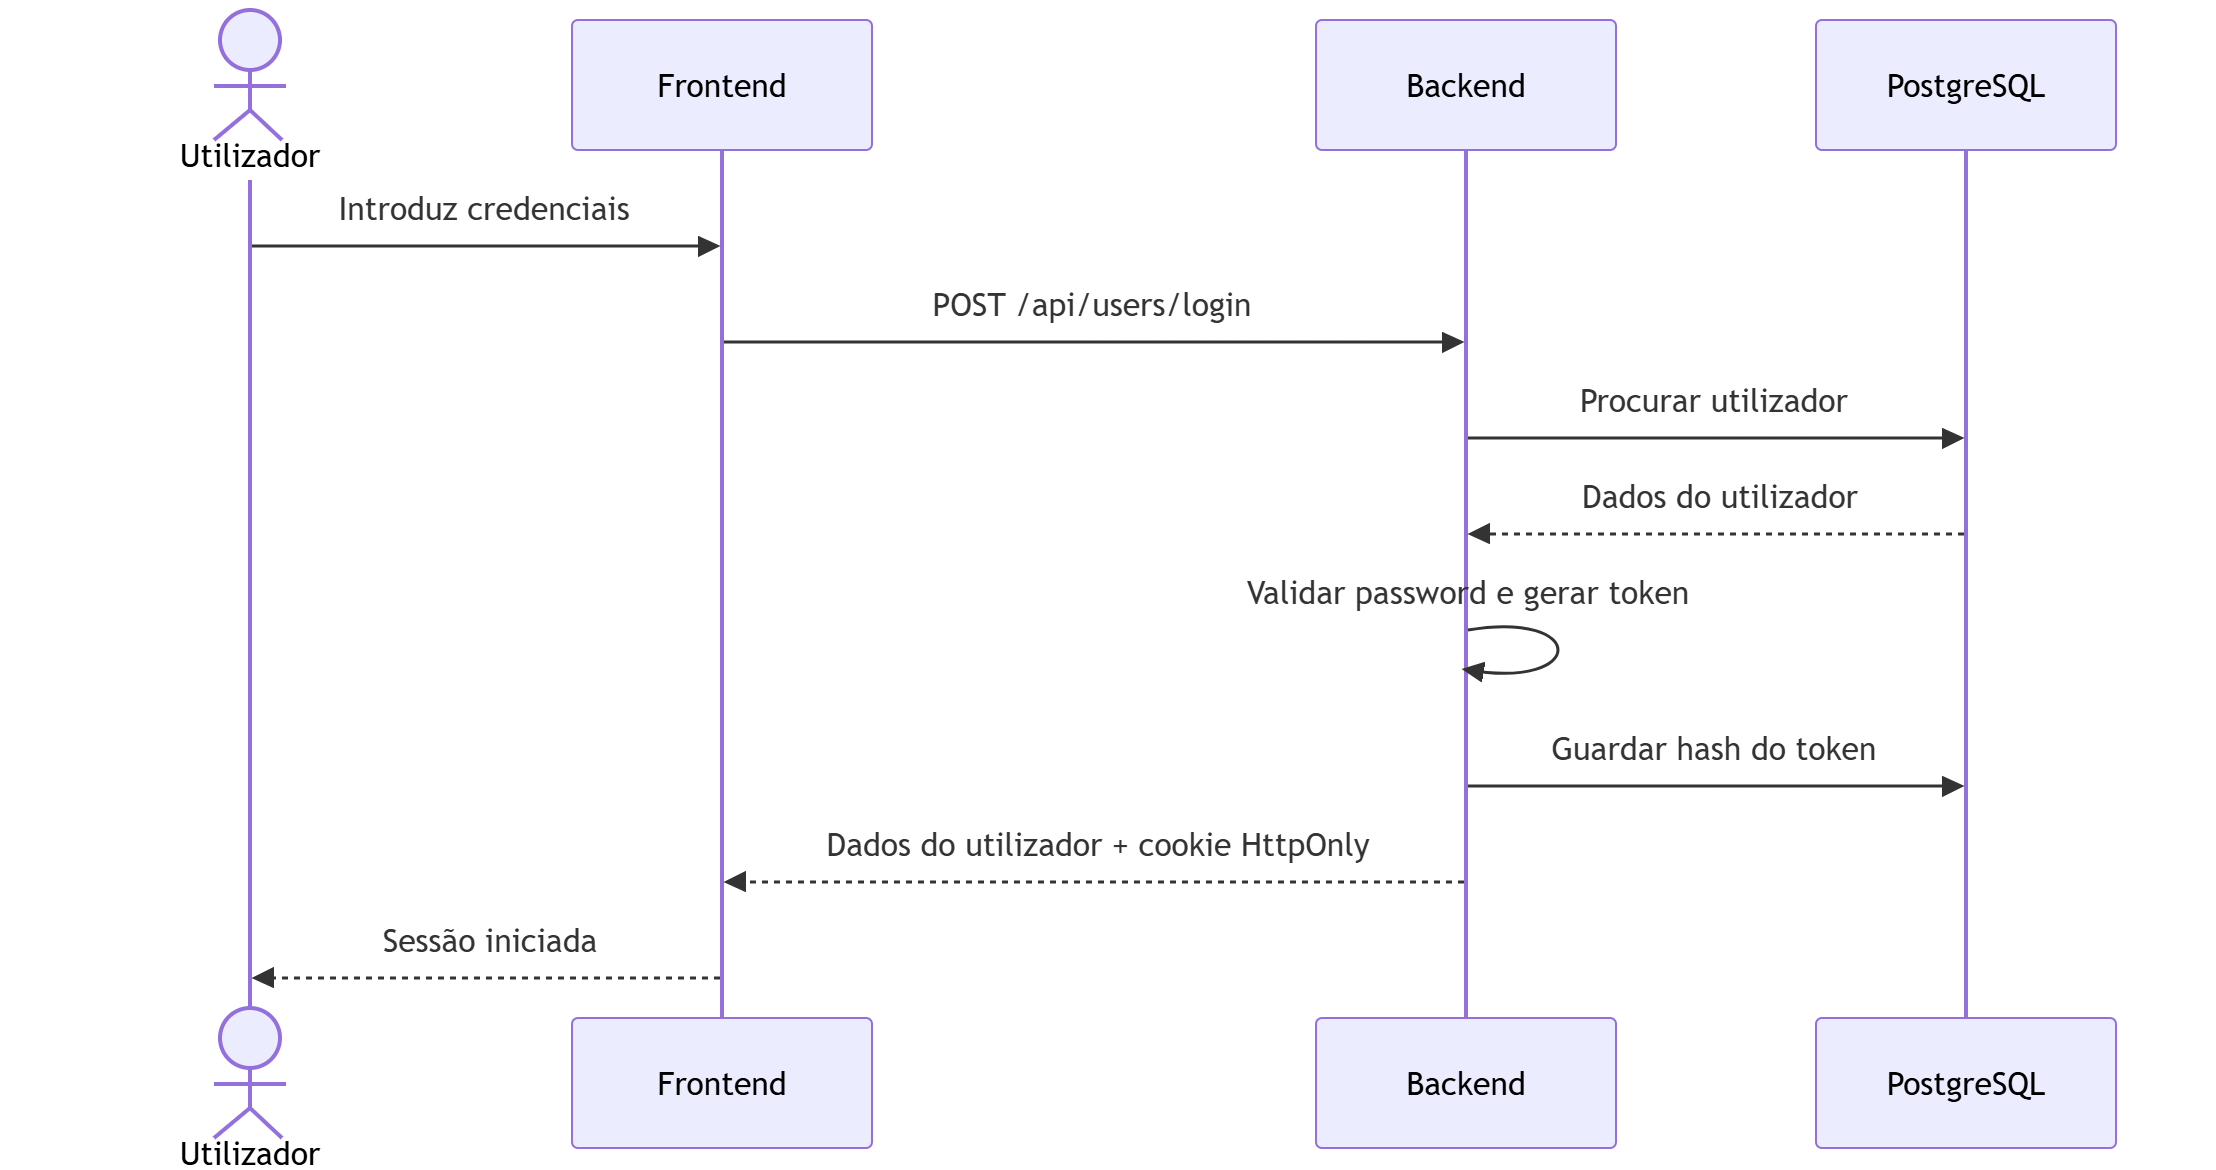
\includegraphics[width=0.9\textwidth]{./figures/auth-flow.png}
    \caption{Fluxo de autenticação}
    \label{fig:auth-flow}
\end{figure}

\subsection{Fluxo de Inscrição de Sócio}

A adesão de sócio é um dos fluxos centrais da aplicação. O utilizador preenche
um formulário no \textit{frontend}, que envia os dados para a API. O
\textit{backend} valida os dados, cria o registo de sócio em estado pendente e
disponibiliza-o para análise pela secretaria ou administração.

\begin{figure}[H]
    \centering
    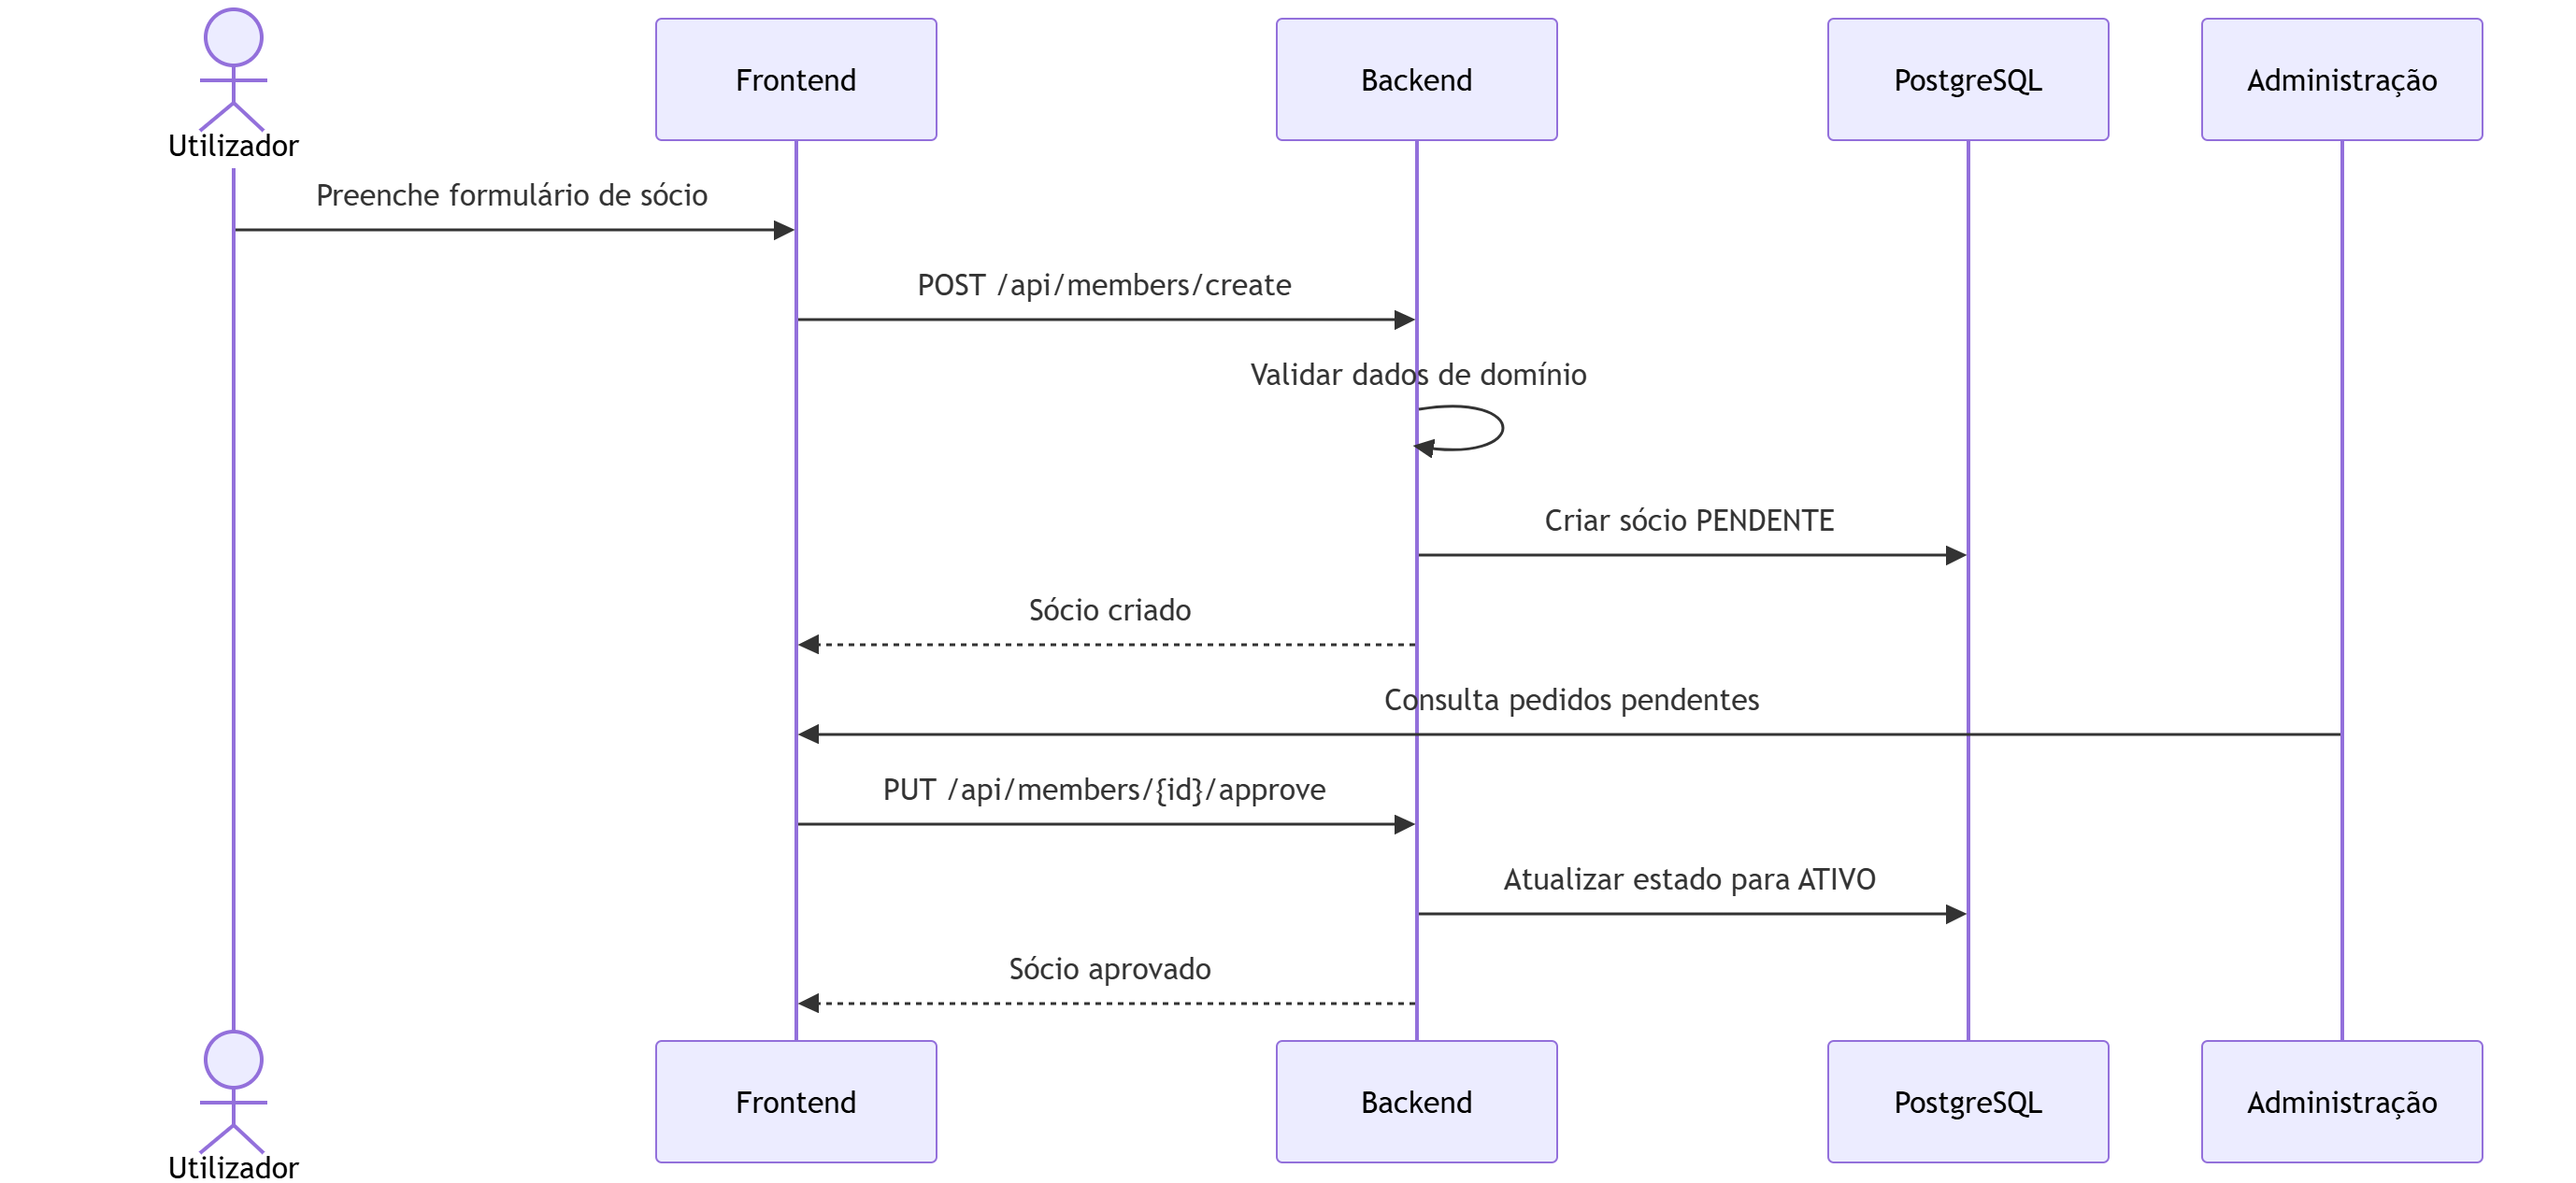
\includegraphics[width=0.9\textwidth]{./figures/member-registration-flow.png}
    \caption{Fluxo de adesão de sócio}
    \label{fig:member-registration-flow}
\end{figure}

\subsection{Fluxo de Inscrição de Atleta}

A inscrição de atleta é mais complexa, uma vez que envolve dados pessoais,
dados desportivos e encarregados de educação. No \textit{backend}, esta
operação cria, numa única transação, o sócio associado, o atleta e os
respetivos encarregados. Esta abordagem garante que não existem atletas
incompletos caso alguma parte da operação falhe.

\begin{figure}[H]
    \centering
    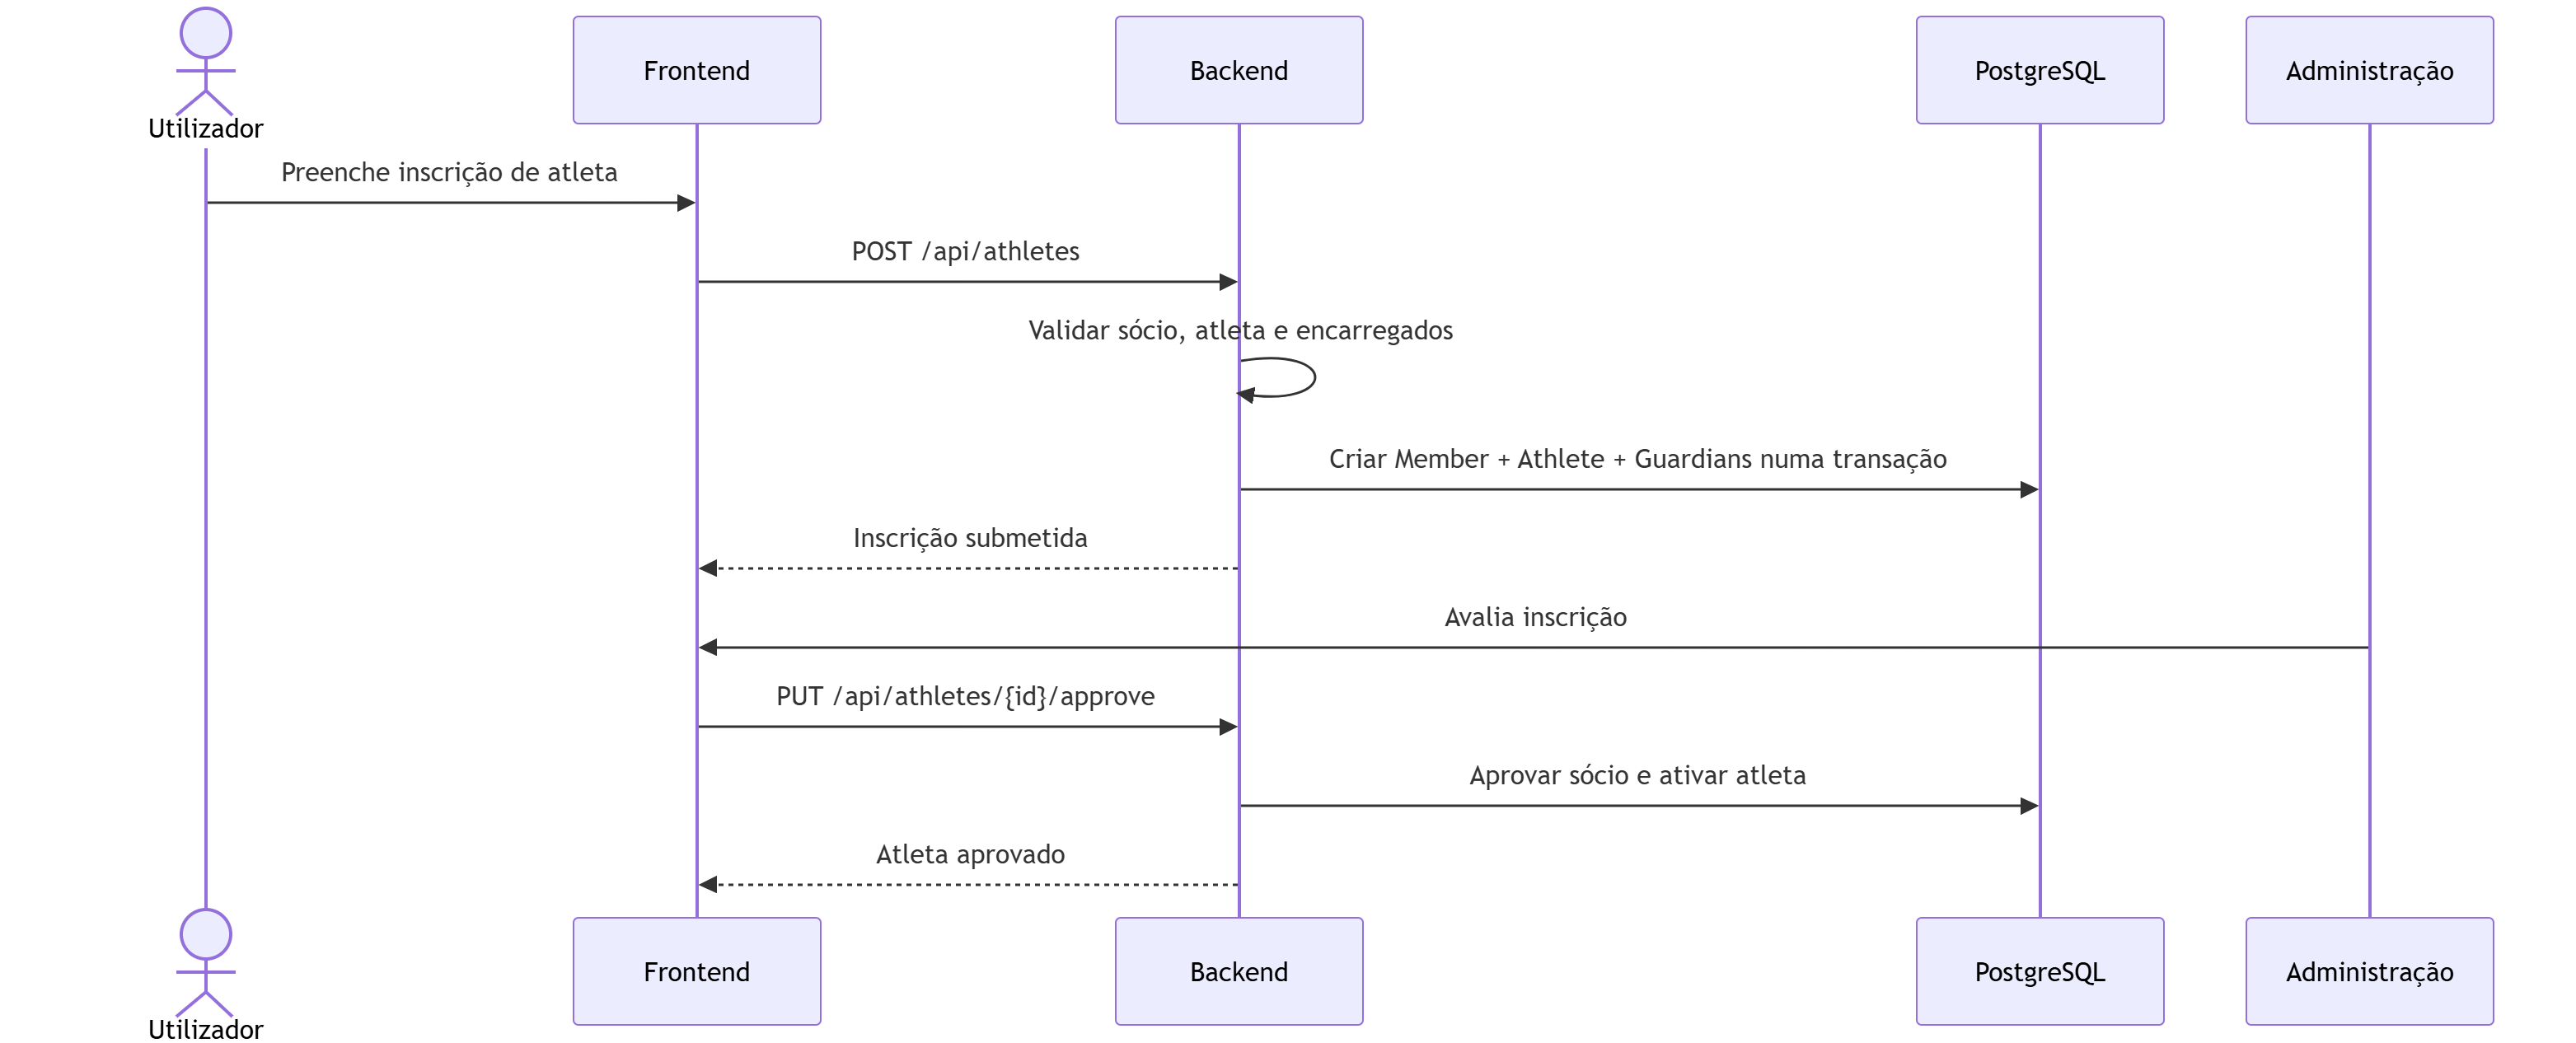
\includegraphics[width=0.9\textwidth]{./figures/athlete-registration-flow.png}
    \caption{Fluxo de inscrição de atleta}
    \label{fig:athlete-registration-flow}
\end{figure}

\subsection{Fluxo de Patrocínio}

No fluxo de patrocínio, o utilizador escolhe uma opção disponível, preenche os
dados do patrocinador e submete o pedido. A secretaria ou administração pode
posteriormente aprovar o pedido, marcar o pagamento e acompanhar o estado do
contrato.

\begin{figure}[H]
    \centering
    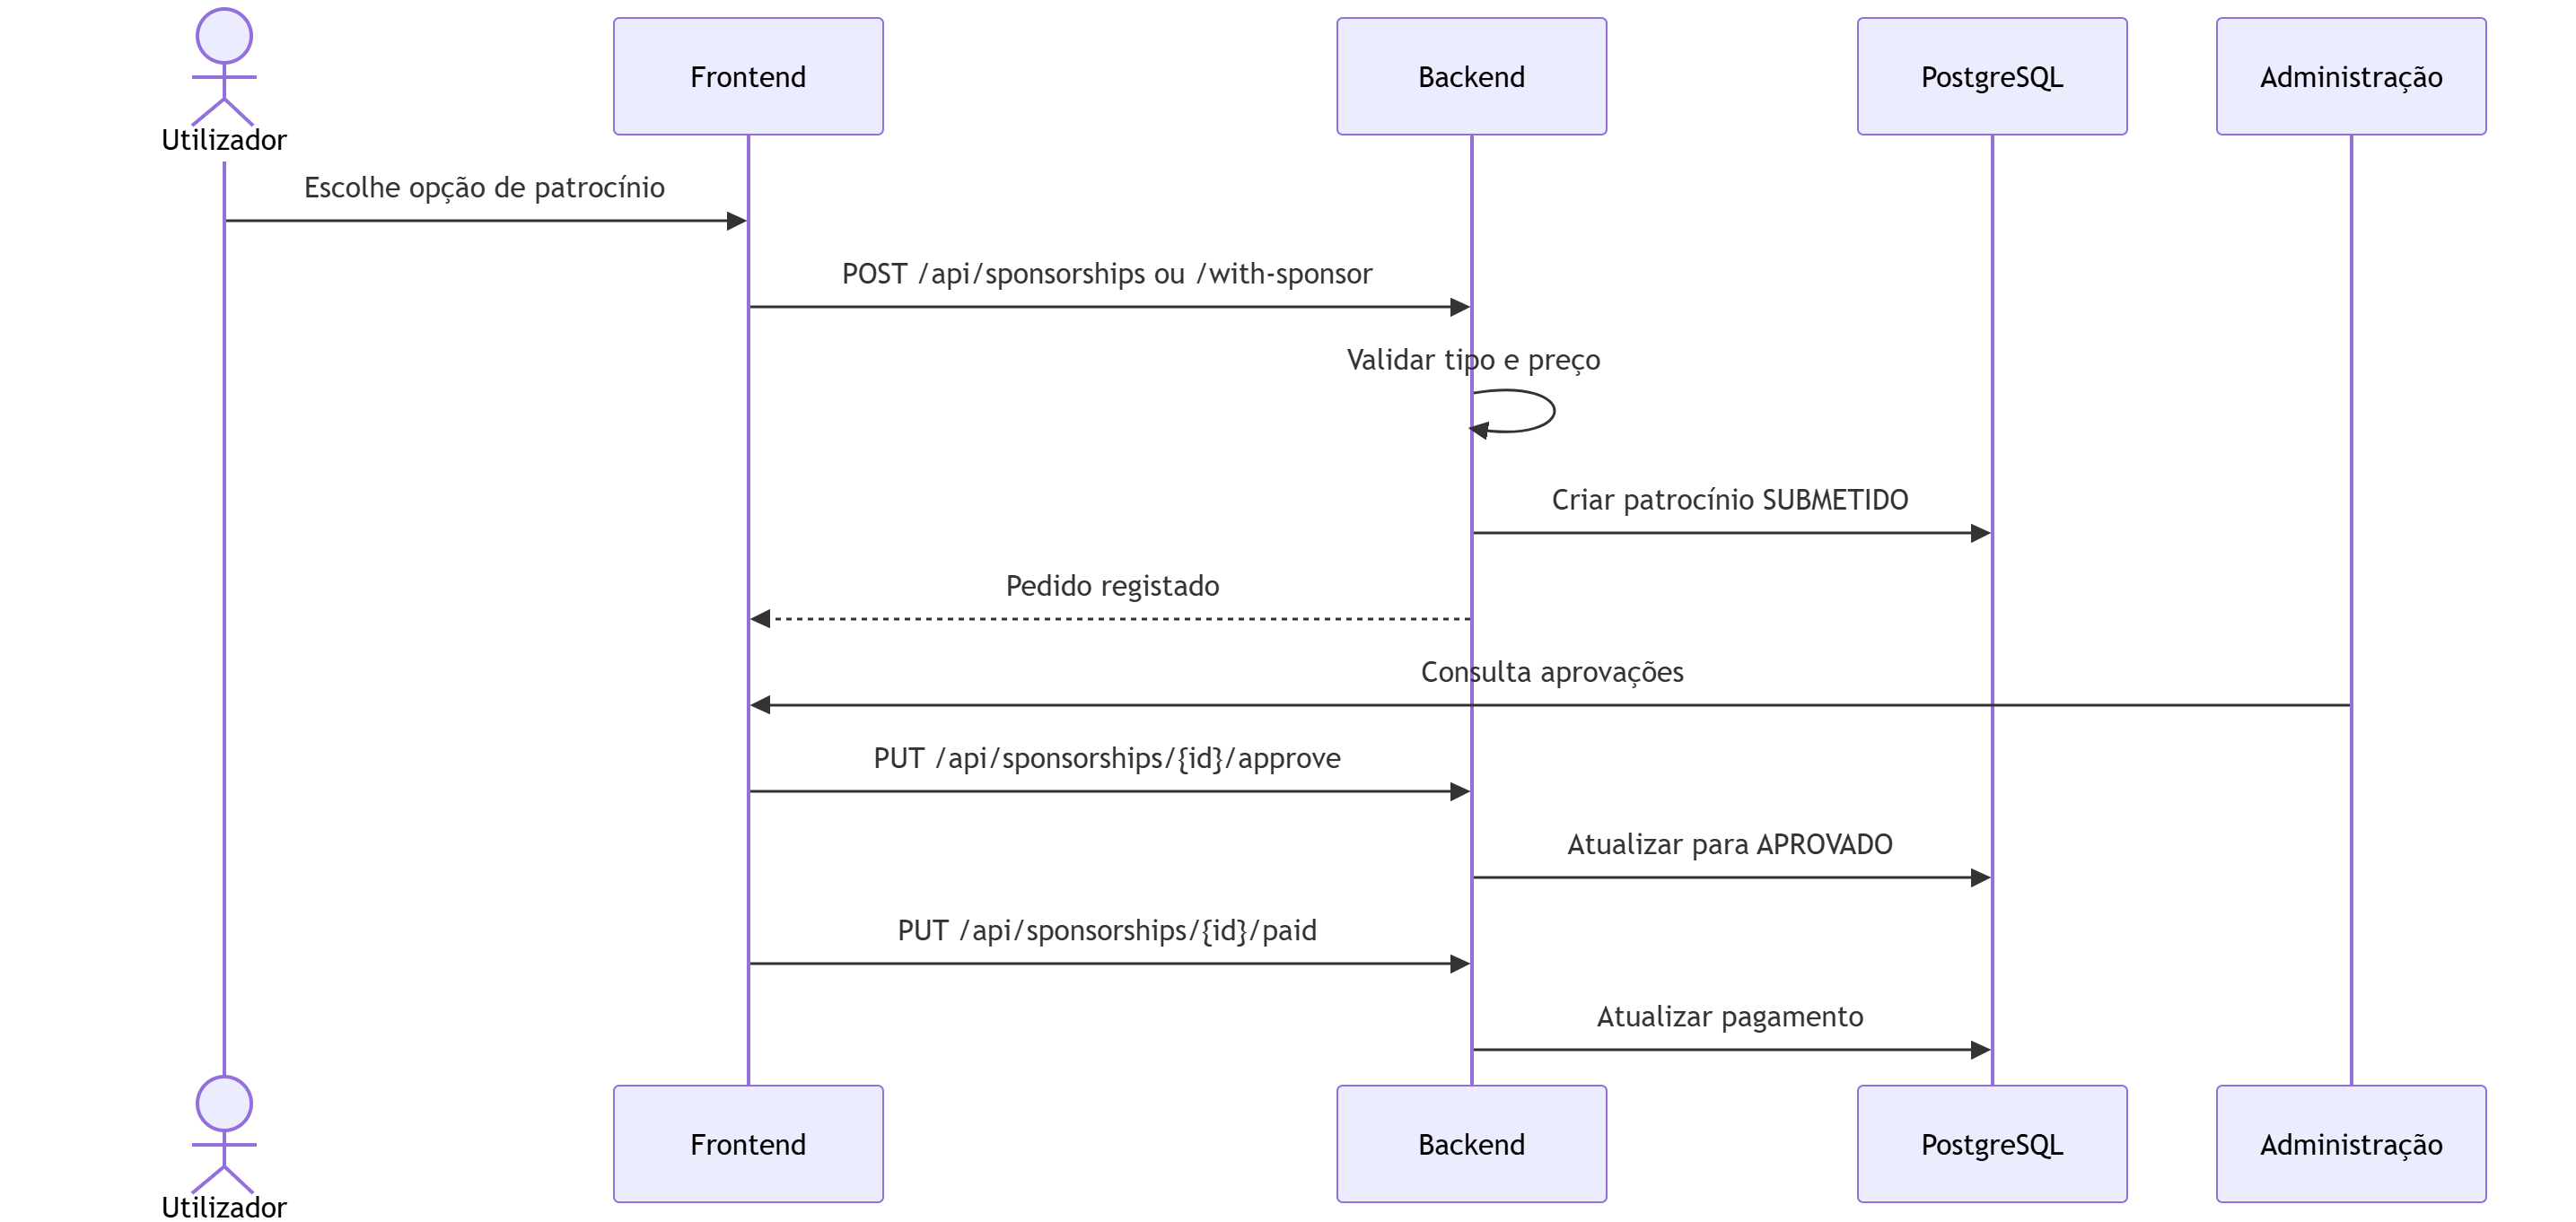
\includegraphics[width=0.9\textwidth]{./figures/sponsorship-flow.png}
    \caption{Fluxo de submissão e aprovação de patrocínio}
    \label{fig:sponsorship-flow}
\end{figure}

\subsection{Fluxo de Compra de Bilhetes}

Na compra de bilhetes, o utilizador seleciona um evento e o setor pretendido.
Quando o bilhete é de sócio, a aplicação valida o número de sócio e a data de
nascimento. Depois é criada uma sessão de pagamento na Stripe. Quando o
pagamento é confirmado, o \textit{backend} confirma os bilhetes, gera os
códigos QR e envia a confirmação por email.

\begin{figure}[H]
    \centering
    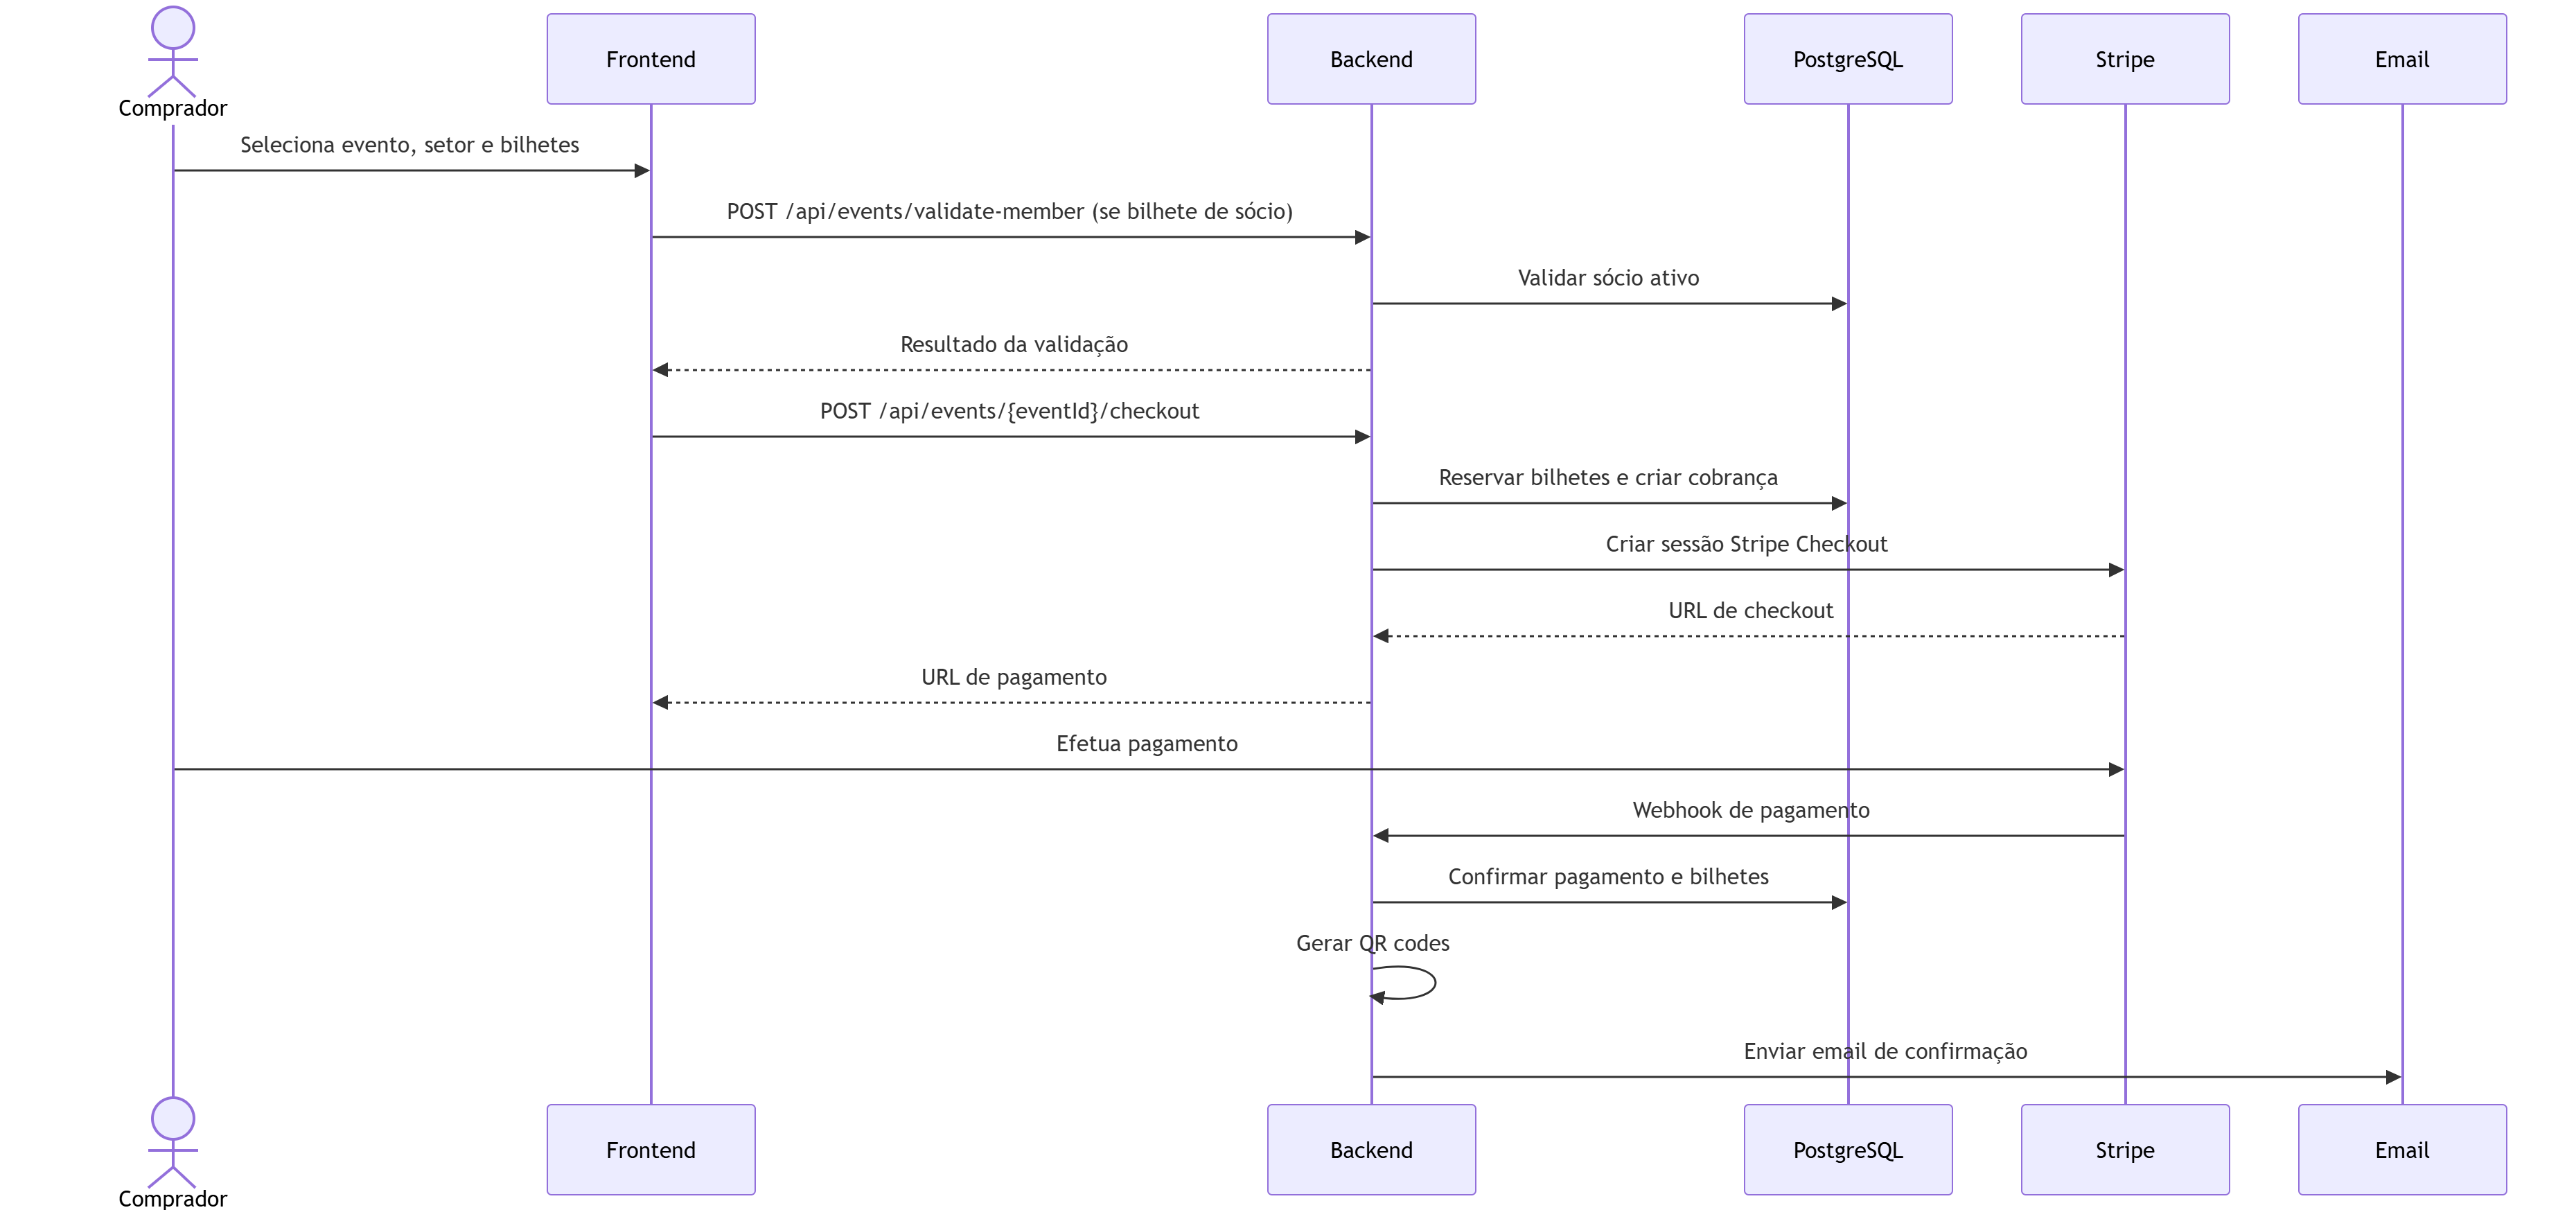
\includegraphics[width=\textwidth]{./figures/ticket-payment-flow.png}
    \caption{Fluxo de compra de bilhetes e confirmação de pagamento}
    \label{fig:ticket-payment-flow}
\end{figure}

\section{Síntese}

A JagozApp foi desenhada para responder a um conjunto alargado de necessidades
de gestão de um clube desportivo local. A separação entre \textit{frontend},
\textit{backend}, base de dados e integrações externas permite organizar o
sistema de forma clara. A adoção de uma arquitetura multi-módulo no
\textit{backend} reforça esta separação, promovendo manutenção, testabilidade
e evolução futura.

Os requisitos definidos cobrem os processos essenciais do clube, desde a gestão
de sócios e atletas até à bilhética, pagamentos, patrocínios e documentos. Os
diagramas apresentados ajudam a compreender como estes processos atravessam as
várias camadas da aplicação e como cada componente contribui para o
funcionamento global do sistema.
